\chapter{State of the Art}
\label{cap:estadoDeLaCuestion}

\section{Gmail API}\label{sect:gmailapi}
In order to be able to read and send emails, it is necessary to access to the user's email data. For this reason, the different ways to obtain this information were studied. One of them is the Gmail API, which allows developers to perform all the actions we need in an easy way.

Gmail API can be used in several programming languages such as Python, PHP, Go, Java, .NET, \ldots Due to the greater number of examples in the starting guides of the Gmail API \citep{gmailAPI} and the previous knowledge that was already had of it, Python was chosen for the first contact with this implement.

The following is a step-by-step explanation of what is necessary to do to access the user's Gmail account, create a message, send an email previously created, create and update a draft, reply a received message (for this it is necessary to know how to create an email) and read important information of message threads and individual emails (such as who is the sender, who will received the message, the subject, the date, the email's body, the attached files, \ldots).

\subsection{OAuth 2.0 Protocol}\label{ssect:oauth}
Gmail API, as it also happens in the case of other Google APIs, uses OAuth 2.0 protocol \citep{oauth} to handle authentication and authorization. As it will be seen later in this section, it is needed to be in possession of OAuth 2.0 client credentials from the Google API Console for having the appropriate permissions to use the Gmail API.

The Google API Console, also known as Google Console Developer\footnote{\url{https://console.developers.google.com/}}, built into Google Cloud Platform, makes possible an authorized access to a user's Gmail data. In order to achieve it, having a Google account is a prerequisite because it will be necessary to access to this platform. Once this web has been accessed, at first we have to create a new development project by clicking in ``New Project'' in the control panel (which is the main tab of the Google Console Developer and the one that opens by default when you access it). When we have already created a project, we will enable the API we are going to work with, in this case the Gmail API. To do this we will look for it in the search engine that we can find in the library of APIs of this platform. Now we can apply for the credentials we need. Accessing to the ``Credentials'' tab and clicking on ``Create Credentials'' will lead us to an easy questionnaire about what type of credentials we prefer that we have to answer by basing on what type of application we are building. Then we must download the .json file and save it in the folder we are going to work in.

Before starting the development of the implementation of the OAuth 2.0 protocol which will provides us a secure and trusted login system to access to the user's Gmail data, we must install the Google Client Library\footnote{\url{https://developers.google.com/gmail/api/downloads}} of our choice of language (as we have said we will use Python for this, so we have to install the libraries \textit{google-api-python-client}, \textit{google-auth-httplib2} and \textit{google-auth-oauthlib}).

There are many ways to obtain the necessary permissions for accessing to the user's emails data following the OAuth 2.0 protocol. As this is a first contact with the Gmail API only with the intention of knowing the possibilities it offers to us and its advantages and disadvantages of using it in our future implementation of our virtual assistant, we are going to develop a simple script which is using a class very useful for local development and applications that are installed on a desktop operating system. The class \textit{InstalledAppFlow}, in \textit{google\_auth\_oauthlib.flow} \citep{oauthlib}, is a \textit{Flow} subclass (which belongs to the same library). Thanks to this last class we have mentioned, \textit{InstalledAppFlow} uses a \textit{requests\_oauthlib.OAuth2Session} instance at \textit{oauth2session} to perform all of the OAuth 2.0 logic. Besides it also inherits from \textit{Flow} the class method \textit{from\_client\_secrets\_file} which creates a \textit{Flow} instance from a Google client secrets file (this file will be the .json file that we obtained through the Google API Console) and a list of OAuth 2.0 Scopes \citep{oauth-scopes}, which are a mechanism  in OAuth 2.0 to limit an application's access to a user's account. An application can request one or more scopes, this information is then presented to the user in the consent screen, and the access token issued to the application will be limited to the scopes granted (we will use the Gmail API OAuth 2.0 Scope which allows us to read, compose, send, and permanently delete all your email).

\begin{figure}[h]
	\centering%
	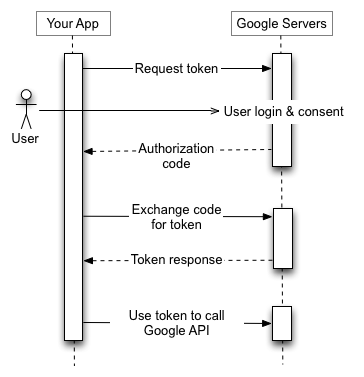
\includegraphics[width = 0.5\textwidth]{Imagenes/Bitmap/webflow.png}%
	\caption{OAuth 2.0 for Web Server Applications and Installed Applications.}%
	Image extracted from \cite{oauth}
	\label{fig:oauth}
\end{figure}

After constructing an \textit{InstalledAppFlow} by calling \textit{from\_client\_secrets\_file} as we have explained, we can invoke the class method \textit{run\_local\_server} which instructs the user to open the authorization URL in the browser and will attempt to automatically open it. This function will start a local web server to listen for the authorization response. Once there is a reply, the authorization server will redirect the user's browser to the local web server. As we can see in \ref{fig:oauth}, the web server will get the authorization code from the response and shutdown, that code is then exchanged for a token.

Then, we will be in possession of the OAuth 2.0 credentials for the user \citep{oauth2.credentials} which we are going to use for accessing the user's Gmail account. In summary, it is possible to obtain the necessary permissions from the user and to follow the OAuth 2.0 protocol, by executing these instructions (written in Python):

\begin{python}
from google_auth_oauthlib.flow import InstalledAppFlow

# Create a flow instance
flow = InstalledAppFlow.from_client_secrets_file('credentials.json', 
	['https://mail.google.com/'])
# Obtain OAuth 2.0 credentials for the user
creds = flow.run_local_server(port = 0)
\end{python}

Now, we are able to call Gmail API by using the token (which is stored in the variable \textit{creds}). However, before starting working on the email data, we should save the OAuth 2.0 credentials since otherwise the user would need to go through the consent screen every time the application is opened. To prevent the latter from happening, to differentiate access from mail management and consequently to reuse as much code as possible; we have implemented the following class \textit{auth}, in \textit{auth.py}, with a main method \textit{get\_credentials}:

\begin{pythonnum}
import pickle
import os.path
from google_auth_oauthlib.flow import InstalledAppFlow
from google.auth.transport.requests import Request
	
class auth:
	def __init__(self, SCOPES, CLIENT_SECRET_FILE):
		self.SCOPES = SCOPES
		self.CLIENT_SECRET_FILE = CLIENT_SECRET_FILE
	
	def get_credentials(self):
		"""
		Obtains valid credentials for accessing Gmail API
		"""
		creds = None
		# The file token.pickle stores the user's access and refresh tokens
		if os.path.exists('token.pickle'):
			with open('token.pickle', 'rb') as token:
				creds = pickle.load(token)
		# If there are no (valid) credentials available, let the user log in
		if not creds or not creds.valid:
			if creds and creds.expired and creds.refresh_token:
				creds.refresh(Request())
			else:
				flow = InstalledAppFlow.from_client_secrets_file(
					self.CLIENT_SECRET_FILE, self.SCOPES)
				creds = flow.run_local_server(port=0)
			# Create token.pickle and save the credentials for the next run
			with open('token.pickle', 'wb') as token:
				pickle.dump(creds, token)
		return creds

\end{pythonnum}

As we can observe in line 17 within \textit{get\_credentials} method, at first we check if the file called \textit{token.pickle} exists, and in that case, it is opened and its information is stored in the variable \textit{creds}. Thus, we avoid to force the user to open the authorization screen. By contrast, as we have seen before, if it does not exists, we obtain the credentials by calling the class methods \textit{from\_client\_secrets\_file} and \textit{run\_local\_server} (it is written between lines 25 and 30).

There is another case that is also reflected in the code above (in lines 23 and 24): the credentials are expired (it is possible to check it by executing \textit{creds.expired}) and they can be refreshed (the OAuth 2.0 refresh token is \textit{creds.refresh\_token}) \citep{oauth2.credentials}. In this situation, we will refresh the access token by invoking the method known as \textit{refresh} and by giving it a \textit{Request} object \citep{request-lib} from \textit{google.auth.transport.requests} as the function parameter which used to make HTTP requests.

\subsection{Building a Gmail Resource}
At this point, with the OAuth 2.0 credentials, we are able to call the Gmail API. For this purpose, it is necessary to construct a resource \citep[/v1/reference]{gmailAPI} for interacting with the API. The \textit{build} method, from \textit{googleapiclient.discovery} library \citep{build-module}, create that object. As we will see later, this resource will lead us to manage emails, drafts, threads and everything we will like to do with the user's Gmail data. This is why, using the \textit{auth.py} file explained in \ref{ssect:oauth}, we are going to start every user session with the instructions below (or their equivalents in the language we are using):

\begin{python}
from googleapiclient.discovery import build
import auth

SCOPES = ['https://mail.google.com/']
CLIENT_SECRET_FILE = 'credentials.json'

# Creation of an auth instance
authInst = auth.auth(SCOPES, CLIENT_SECRET_FILE)
# Constructing the resource API object
service = build('gmail', 'v1', credentials = authInst.get_credentials())
\end{python}

Henceforth, we will use the \textit{service} variable to relate it with the resource object created by the \textit{build} method.

\subsection{Users resource}\label{ssect:userres}
The \textit{build} method could be called for obtaining any resource of any Google API (by giving it the suitable parameters). Our specific \textit{service} created\footnote{\url{http://googleapis.github.io/google-api-python-client/docs/dyn/gmail\_v1.html}} has an important instance method that we are going to invoke for every execution: \textit{users()} method. It returns what is known as users resource \citep[/v1/reference/users]{gmailAPI}.

The users resource has also instance methods, which return other Gmail API resources that we are going to need, such as \textit{drafts()}, \textit{labels()}, \textit{messages()} and \textit{threads()} which return drafts, labels, messages and threads resources respectively. Moreover, it possesses the three methods that we explain hereunder (we must remember that for being able to execute any method that we are going to explain in this and next sections, it is necessary to have the appropriate authorization with at least one of the required scopes that we can look up in its documentation):

\begin{itemize}
	\item\textit{getProfile(userId)}: it returns an object with a dictionary structure as it follows:
	\begin{python}
	{
	'threadsTotal' : integer, # Total number of threads in the mailbox
	'emailAddress' : string, # User's email address
	'historyId' : string, # ID of the mailbox's current history record
	'messagesTotal' : integer # Total number of messages in the mailbox
	}
	\end{python}
	The parameter is a string with the user's email address. If we remember the authentication process, at no time we ask the user about the email address because we decided to let the Google API functions to handle all that procedure. Therefore we have no way to know this information. Nevertheless, the special string value \textit{'me'} can be used to indicate the authenticated user. For knowing the required scopes for invoking this function look up in \cite[/v1/reference/users/getProfile]{gmailAPI}.
	\item\textit{stop(userId)}: stop receiving push notifications for the given user mailbox. As it happens with \textit{getProfile}, the parameter is a string with the user's email address, but it is possible to use the especial string value \textit{'me'}.
	\item\textit{whatch(userId, body)}: set up or update a push notification watch on the given user mailbox.
\end{itemize}

As we are going to call only the \textit{getProfile} method, we have described on details this first function and we have just given an idea about what the rest of them do. Now, in next sections, we are going to explain all the resources we can create with the user resource.

\subsection{Labels resource}\label{ssect:labres}
As we have seen in the explanation of users resource (section \ref{ssect:userres}), we can obtain labels resource \citep[/v1/reference/users/labels]{gmailAPI} by invoking \textit{labels()} instance method of our users resource, that is to say, by using our \textit{service} variable, the instruction \textit{service.users().labels()} will return the label resource.

Labels are used to categorize messages and threads within the user's mailbox. They have a dictionary structure and their representation is what we can observe hereunder:

\begin{python}
{
'id' : string, # The immutable identifier of the label
'name' : string, # The display name
# The visibility of messages in the Gmail web interface
'messageListVisibility' : string,
'labelListVisibility' : string, # The visibility of label
'type' : string, # The owner type of the label ('system' or 'user')
'messagesTotal' : integer, # Total number of messages with the label
'messagesUnread' : integer, # Number of unread messages with the label
'threadsTotal' : integer, # Total number of threads with the label
'threadsUnread' : integer, # Number of unread threads with the label
'color' : {
	'textColor' : string, # Text color of the label, represented as hex string
	'backgroundColor' : string # Background color represented as hex string #RRGGBB
	}
}
\end{python}

The important fields we are going to need are the \textit{name} and the \textit{type}. Labels with \textit{system} type, such as \textit{INBOX}, \textit{SENT}, \textit{DRAFTS} and \textit{UNREAD}, are internally created and cannot be added, modified or deleted.

In order to obtain a label object, we will use the methods of this resource: create, delete, get, list, patch and update. In this manner, for example, we can store a label object by calling the next instructions:

\begin{python}
labels = service.users().labels()
labelList = labels.list(userId = 'me').execute()
label = labels.get(id = labelList[0]['id'], userId = 'me')
\end{python}

It is necessary to use the \textit{get} method because, as we can look up in \cite[/v1/reference/users/labels/list]{gmailAPI}, the \textit{list} method only contains an \textit{id}, \textit{name}, \textit{messageListVisibility}, \textit{labelListVisibility} and \textit{type} of each label.

\subsection{Messages resource}
In most of the operations we are going to execute, it will be essential the correct management of messages. Therefore, knowing how the emails are represented in Gmail API and how to use them is imperative to understand how to work with this API. For this reason, in this section we are going to delve into the messages resource of the Gmail API, its structure and its methods. As we saw in section \ref{ssect:userres}, we can access to this resource by invoking the \textit{messages()} method when we have a users resource.

\subsubsection{Resource representation}

Regardless of which programming language is used, messages resource \citep[/v1/reference/users/messages]{gmailAPI} internally has a dictionary structure as we can see down below:

\begin{python}
{
'id' : string,
'threadId' : string,
'labelIds' : [ string ],
'snippet' : string,
'historyId' : unsigned long,
'internalDate' : long,
'payload' : {
	'partId' : string,
	'mimeType' : string,
	'filename' : string,
	'headers' : [
		{
		'name' : string,
		'value' : string
		}
	],
	'body' : users.messages.attachments resource,
	'parts' : [ (MessagePart) ]
	},
'sizeEstimate' : integer,
'raw' : bytes
}
\end{python}

The more important keys (for us) of this data structure are (at least the most useful keys for our purpose):
\begin{itemize}
	\item\textit{id}: an immutable string which identifies the message.
	\item\textit{threadId}: we will explain the thread resource in \ref{ssect:threads} and we will see that a thread is composed of different messages that share common characteristics. The value of this field is a string which represent the identifier of the thread the message belongs to.
	\item\textit{labelIds}: a list of the identifiers of labels (see section \ref{ssect:labres}) applied to the message.
	\item\textit{payload}: as we can see in the resource representation above, it has a dictionary data structure. The \textit{payload} field is the parsed email structure in the message parts. The more important keys of the \textit{payload} field are:
	\begin{itemize}
		\item\textit{headers}: a list of headers. It contains the standard RFC 2822 \citep{rfc2822} email headers such as \textit{To}, \textit{From}, \textit{Subject} and \textit{Date}. Each header has a \textit{name} field, which is the name of the header (for example \textit{From}), and a \textit{value} field, which is the value of the header (following the same example as with the \textit{name} field: \textit{example@gmail.com} could be the value).
		\item\textit{parts}: a list which contains the different child MIME message parts (we will delve into this field in section \ref{sssect:mime}).
	\end{itemize}
	\item\textit{raw}: the entire email message in an RFC 2822 \citep{rfc2822} formatted and base64url (see section \ref{sssect:base64}) encoded string.
\end{itemize}

\subsubsection{Methods}
As any other resource we have studied and we will study, messages resource has a lot of methods, many of whom we are going to call for our purposes. We will limit ourselves to describing the methods we are going to use:

\begin{itemize}
	\item\textit{attachments()}: returns the attachments resource (see section \ref{ssect:attres})
	\item\textit{get(userId, id, format = 'full', metadataHeaders = None)}: if successful, this method returns the requested messages resource. Its parameters are:
	\begin{itemize}
		\item\textit{id}: the identifier string of the message to retrieve.
		\item\textit{userId}: the user's email address. As it happens with the \textit{getProfile} method of the users resource (see section \ref{ssect:userres}), the special string value \textit{'me'} can be used to indicate the authenticated user.
		\item\textit{format} (optional parameter): the format to return the message in. Acceptable values are: \textit{'full'} (return the full email data with body content parsed in the \textit{payload} field and the \textit{raw} field is not used), \textit{'metadata'} (returns only email message identifier, labels and email headers), \textit{'minimal'} (returns only email message identifier and labels) and \textit{'raw'} (returns the full email message data with the body content in the \textit{raw} field as a base64url (see section \ref{sssect:base64}) encoded string and the \textit{payload} field is not used).
		\item\textit{metadataHeaders} (optional parameter): it is only used when the format parameter takes the punctual value of \textit{'metadata'}. It is a string list where we have to insert the headers we want to be included.
	\end{itemize}
	For knowing the required scopes for invoking this function look up in \cite[/v1/reference/users/messages/get]{gmailAPI}
	\item\textit{list(userId, includeSpamTrash = false, labelIds = None, maxResults = None, pageToken = None, q = None)}: returns a resource with the following structure:
	\begin{python}
		{
		'messages' : [ users.messages resource ],
		'nextPageToken' : string,
		'resultSizeEstimate' : unsigned integer
		}
	\end{python}
	As it happens with the \textit{list} method of the labels resource (see section \ref{ssect:labres}), \textit{'messages'} list does not contain all of a message information (for obtaining the full email data we can use \textit{get} method). Each element of this list only contains the \textit{id} and \textit{threadId} field.
	
	The parameters of this method are:
	\begin{itemize}
		\item\textit{userId}: user's email address (we can use the special string value \textit{'me'}).
		\item\textit{includeSpamTrash} (optional parameter): boolean parameter which determines if it includes messages with the labels \textit{SPAM} and \textit{TRASH} in the result of the operation.
		\item\textit{labelIds} (optional parameter): it is a list which let us filter the messages by only returning emails with labels that match all of the identifiers that belong to this list.
		\item\textit{maxResults} (optional parameter): an integer which determines the maximum number of messages to return.
		\item\textit{pageToken} (optional parameter): string which specifies a page of results.
		\item\textit{q} (optional parameter): string which let us do an specific query (with the same query format as the Gmail search box) and filter the messages by only returning emails that match with it.
	\end{itemize}
	For knowing the required scopes for invoking this function look up in \cite[/v1/reference/users/messages/list]{gmailAPI}
	\item\textit{send(userId, body = None, media\_body = None, media\_mime\_type = None)}: 
\end{itemize}

\subsubsection{MIME} \label{sssect:mime}

\subsubsection{Base64} \label{sssect:base64}

\subsection{Attachments resource} \label{ssect:attres}

\subsection{Threads resource}\label{ssect:threads}